\scanpage{77}
% archive foliation: 76
% upper-left diagram
\diagram{\begin{tikzcd}[ampersand replacement=\&,column sep=small]
\&R\arrow[dl,"p"']\arrow[d,bend right=16,"q'"']\arrow[d,bend left=16,"q''"]\arrow[dr,"r"]\&\\
S\&A\&F
\end{tikzcd}}
% upper-centre diagram
\diagram{\begin{tikzcd}[ampersand replacement=\&,column sep=large]
\&R^{\unsure{o|0}}=R\arrow[dl,"p^{\unsure{o|0}}=p"']\arrow[d,bend right=16,"q'^{\unsure{o|0}}=q''"']\arrow[d,bend left=16,"{q''^{\unsure{o|0}}=\deleted{\unsure{q'}}\inserted{q'\circ\sigma_2}}"]\arrow[dr,"{\unsure{q^{o}|r^{o}}=q\circ\sigma_2}"]\&\\
S\&A\&F
\end{tikzcd}}
% upper-middle triangle drawing
\figure{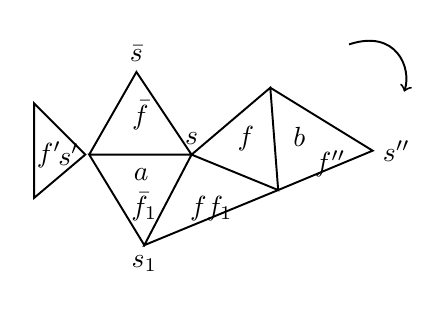
\begin{tikzpicture}[x=1cm,y=1cm,line width=.7pt]
\coordinate (s) at (2,1);\coordinate (sp) at (.7,1);\coordinate (sb) at (1.3,2.05);\coordinate (sone) at (1.4,-.15);\coordinate (r) at (3.1,.55);\coordinate (t) at (3,1.85);\coordinate (spp) at (4.3,1.05);
\draw (0,.45)--(.65,1)--(0,1.65)--cycle;
\draw (sp)--(sb)--(s)--(sp)--(sone)--(s)--(t)--(r)--(s)--(sone)--(r)--(spp)--(t);
\node at (.19,1) {$f'$};\node[left] at (sp) {$s'$};\node[above] at (sb) {$\bar s$};\node[above] at (s) {$s$};\node[below] at (sone) {$s_1$};\node[right] at (spp) {$s''$};
\node at (1.35,1.5) {$\bar f$};\node at (1.36,.75) {$a$};\node at (1.4,.34) {$\unsure{\bar f_1}$};\node at (2.69,1.2) {$f$};\node at (3.37,1.23) {$b$};\node at (3.76,.88) {$f''$};\node at (2.25,.32) {$\deleted{\unsure{f}}f_1$};
\draw[->] (4,2.4) .. controls (4.6,2.6) and (4.8,2.1) .. (4.7,1.8);
\end{tikzpicture}}
% middle-left formulae
\[\begin{aligned}
p(s,f)&=s&\sigma_0(s,f)&=(s',f')\\
r(s,f)&=f&\sigma_2(s,f)&=(s'',f'')\\
q'(s,f)&=a\\
q''(s,f)&=b
\end{aligned}\]
\[\sigma_0\sigma_2(s',f')=\sigma_2\sigma_0(s',f')=(s'',f'')\]
% upper-right display, right edge unclosed in the scan
\[E=(R,q')\times_A(R,q'')=
\left\{\overbrace{((s,f),(\bar s,\bar f))}^{\text{\unsure{rempl.}}\ (s,a,\bar f)}\mid q'(s,f)=q''(\bar s,\bar f)\right.\]
\margin{$\unsure{''}$}
% small diagram below E
\diagram{\begin{tikzcd}[ampersand replacement=\&,column sep=small]
\&E\arrow[dl,"\pi_{01}"']\arrow[d,"\pi_{02}"]\arrow[dr,"\pi_{12}"]\&\\
R\&R\&R
\end{tikzcd}}
% middle-right displays
\[\begin{aligned}
\pi_{01}^{+}(s,f,\bar s,\bar f)&=(s,f)\\
\pi_{12}^{+}(s,f,\bar s,\bar f)&=(\bar s,\bar f)\\
\pi_{02}^{+}(s,f,\bar s,\bar f)&=(s,\bar f)
\end{aligned}\]
\[E^+=\left\{(s,f,\bar s,\bar f\unsure{]|)}\in E\mid(s,a,\bar f)\ \text{\unsure{direct}}\right.\]
\inserted{$a=q'(s,f)=q''(\bar s,\bar f)$}
% three formulae above fold
\[\left\{\begin{aligned}
\sigma_0(s,f,\bar s,\bar f)&=(s,\unsure{f_2'|f_2},\bar s,\bar f)\\
\sigma_1(s,f,\unsure{\bar s_1|\bar s},\unsure{\bar f_2|\bar f})&=(s,f_1,\unsure{\bar s'|\bar s_1},\bar f)\\
\sigma_2(s,f,\bar s,\bar f)&=(s,f,\bar s_1,\unsure{f_1|\bar f_1})
\end{aligned}\right.\]
% bottom-left diagram
\diagram{\begin{tikzcd}[ampersand replacement=\&,column sep=small,row sep=large]
\&E^+\arrow[dl,"\pi_{01}^{+}"']\arrow[d,"\pi_{02}^{+}"]\arrow[dr,"\pi_{12}^{+}"]\&\\
R\&R\&R\\
\&E^-\arrow[ul,"\pi_{01}^{-}"]\arrow[u,"\pi_{02}^{-}"]\arrow[ur,"\pi_{12}^{-}"']\&
\end{tikzcd}}
% bottom-right isolated diagram objects
\diagram{\begin{tikzcd}[ampersand replacement=\&,row sep=huge]E^+\\E^-\end{tikzcd}}
